\documentclass[a4paper,onecolumn,oneside,11pt,wide,floatssmall]{mwrep}
\usepackage[MeX]{polski}
\usepackage[utf8]{inputenc}
\usepackage{amssymb}
\usepackage[polish]{babel}

\let\emptyset\varnothing

\usepackage{bookman}
\usepackage[T1]{fontenc}

\usepackage{hyperref}
\usepackage{url}
\usepackage{breakurl}

\usepackage{wrapfig}
\usepackage{graphicx}
\usepackage{epstopdf}

\usepackage{units}

\usepackage{listings}
\lstset{language=C}
\renewcommand*\lstlistingname{Wydruk}
\renewcommand*\lstlistlistingname{Spis wydruków}


\usepackage[chapter]{algorithm}
\makeatletter
\renewcommand{\ALG@name}{Algorytm}
\renewcommand{\listalgorithmname}{Lista algorytmów}
\renewcommand{\thealgorithm}{\arabic{chapter}.\arabic{algorithm}.}
\makeatother

%% \usepackage[noend]{algorithmic}
\usepackage[noend]{algpseudocode}
%\algsetup{indent=2em}
\renewcommand{\algorithmicrequire}{\textbf{Wymaga:}}
\renewcommand{\algorithmicensure}{\textbf{Zapewnia:}}
\renewcommand{\algorithmiccomment}[1]{{\footnotesize \it \{ #1 \}}}
\renewcommand{\algorithmicif}{\textbf{Jeżeli}}
%% \renewcommand{\algorithmicthen}{\textbf{wówczas}}
\renewcommand{\algorithmicthen}{}
\renewcommand{\algorithmicelse}{\textbf{wpp.}}
%\renewcommand{\algorithmicelsif}{\algorithmicelse \textbf{jeżeli}}
\renewcommand{\algorithmicfor}{\textbf{Dla}}
\renewcommand{\algorithmicforall}{\textbf{Dla wszystkich}}
%% \renewcommand{\algorithmicdo}{\textbf{wykonuj}}
\renewcommand{\algorithmicdo}{\textbf{}}
\renewcommand{\algorithmicwhile}{\textbf{Dopóki}}
\renewcommand{\algorithmicloop}{\textbf{Wykonuj}}
\renewcommand{\algorithmicrepeat}{\textbf{Wykonuj}}
\renewcommand{\algorithmicreturn}{\textbf{Zwróć}}
\renewcommand{\algorithmicuntil}{\textbf{aż}}
\renewcommand{\algorithmicfunction}{\textbf{Funkcja}}
\renewcommand{\algorithmicprocedure}{\textbf{Procedura}}


\usepackage{geometry}
\textwidth\paperwidth
\advance\textwidth -55mm
\oddsidemargin-0.9in
\advance\oddsidemargin 33mm
\evensidemargin-0.9in
\advance\evensidemargin 33mm
\topmargin -1in
\advance\topmargin 25mm
\setlength\textheight{48\baselineskip}
\addtolength\textheight{\topskip}
\marginparwidth15mm

\clubpenalty=10000
\widowpenalty=10000
\brokenpenalty=10000
\sloppy

\tolerance4500
\pretolerance250
\hfuzz=1.5pt
\hbadness1450

\renewcommand{\chaptermark}[1]{\markboth{\scshape\small\bfseries \
#1}{\small\bfseries \ #1}}
\renewcommand{\sectionmark}[1]{\markboth{\scshape\small\bfseries\thesection.\
#1}{\small\bfseries\thesection.\ #1}}
\newcommand{\headrulewidth}{0.5pt}
\newcommand{\footrulewidth}{0.pt}
\pagestyle{uheadings}

\usepackage{color,graphicx}

\usepackage[sort,compress]{cite}

\newcommand{\TODO}[1]{{\setlength{\fboxsep}{0pt}\tiny (\colorbox{red}{TODO}: #1)}}
\newcommand{\ang}[1]{ang.\ {\it #1}}

\usepackage{titling}
\title{Alokacja ciągłych fizycznie obszarów pamięci w~systemie Linux}
\author{Michał Nazarewicz}
\date{\today}
\newcommand{\theengishtitle}{Physically contiguous memory alloction in Linux-based systems}


\begin{document}

\pagenumbering{roman}
\renewcommand{\baselinestretch}{1.0}
\raggedbottom

\begin{titlepage}
    % Strona tytułowa
    \vbox to\textheight{\hyphenpenalty=10000
    \begin{center}
        \begin{tabular}{p{107mm} p{9cm}}
            \begin{minipage}{9cm}
              \begin{center}
              Politechnika Warszawska \\
              Wydział Elektroniki i~Technik Informacyjnych \\
              Instytut Informatyki
              \end{center}
            \end{minipage}
            &
            \begin{minipage}{8cm}
            \begin{flushleft}
             \footnotesize
              Rok akademicki 2012/2013
            \vspace*{2.75\baselineskip}
            \end{flushleft}
            \end{minipage} \\
        \end{tabular}
        \vspace*{3.75\baselineskip}
        \par\vspace{\smallskipamount}
        \includegraphics[width=4cm]{build/pw.eps}\par
        \vspace*{2\baselineskip}{\LARGE Praca dyplomowa inżynierska\par}
        \vspace{3\baselineskip}{\LARGE\strut \theauthor\par}
        \vspace*{2\baselineskip}{\huge\bfseries \thetitle\par}

        \vspace*{7\baselineskip}
        \hfill\mbox{}\par\vspace*{\baselineskip}\noindent
        \begin{tabular}[b]{@{}p{3cm}@{\ }l@{}}
            {\large\hfill } & {\large }
        \end{tabular}
        \hfill
        \begin{tabular}[b]{@{}l@{}}
        Opiekun pracy: \\[\smallskipamount]
        {\large dr inż.\ Wojciech Zabołotny}
        \end{tabular}\par
        \vspace*{4\baselineskip}
    \begin{tabular}{p{\textwidth}}
    \begin{flushleft}
        \begin{minipage}{7cm}
        Ocena \dotfill
        \par\vspace{1.6\baselineskip}
        \dotfill
        \par\noindent
        \centerline{\footnotesize Podpis Przewodniczącego} \par
        \centerline{\footnotesize Komisji Egzaminu Dyplomowego}\par
        \end{minipage}
    \end{flushleft}
    \end{tabular}
    \end{center}}

    % Życiorys
    \newpage\thispagestyle{empty}
    \begin{tabular}{p{5cm} p{12cm}}
    \begin{minipage}{5cm}
    \center
    \IfFileExists{bsc-photo.eps}{
      \includegraphics[width=4.5cm]{bsc-photo.eps}
    }{
      \includegraphics[width=4.5cm]{build/photo.eps}
    }
    \end{minipage}
    &
    \begin{minipage}{12cm}
    \begin{flushleft}
    \par\noindent\vspace{1\baselineskip}
    \begin{tabular}[h]{l l}
    {\it Kierunek:}       & Informatyka \\[12pt]
    {\it Specjalność:}    & Inżynieria Systemów \\
                          & Informatycznych \\[12pt]
    {\it Data urodzenia:} & 31 sierpnia 1986~r. \\[12pt]
    {\it Data rozpoczęcia studiów:} & 1 lutego 2006 r. \\
    \end{tabular}
    \par\noindent\vspace{1\baselineskip}
    \end{flushleft}
    \end{minipage}
    \end{tabular}
    \vspace*{1\baselineskip}
    \begin{center}
        {\large\bfseries Życiorys}\par\bigskip
    \end{center}

    \IfFileExists{bsc-bio.tex}{\indent\input{bsc-bio}}{
      \begin{center}
        $\ddot\smile$
      \end{center}
    }
    \par
    \vspace{2\baselineskip}
    \hfill\parbox{15em}{{\small\dotfill}\\[-.3ex]
    \centerline{\footnotesize podpis studenta}}\par
    \vspace{3\baselineskip}
    \begin{center}
        {\large\bfseries Egzamin dyplomowy} \par\bigskip\bigskip
    \end{center}
    \par\noindent\vspace{\baselineskip}
    Złożył egzamin dyplomowy w dn. \dotfill
    \par\noindent\vspace{\baselineskip}
    Z wynikiem \dotfill
    \par\noindent\vspace{\baselineskip}
    Ogólny wynik studiów \dotfill
    \par\noindent\vspace{\baselineskip}
    Dodatkowe wnioski i uwagi Komisji \dotfill
    \par\noindent\vspace{\baselineskip}
    \dotfill

    % Streszczenie
    \newpage\thispagestyle{empty}
    \vspace*{2\baselineskip}
    \begin{center}
        {\large\bfseries Streszczenie}\par\bigskip
    \end{center}

    {\itshape Wiele podzespołów komputera, a~szczególnie
      tzw.\ systemów wbudowanych, jest zazwyczaj podłączonych
      bezpośrednio do magistrali systemowej, przez co muszą operować
      adresami fizycznymi.  Równocześnie mechanizmy bezpośredniego
      dostępu do pamięci (\ang{Direct Memory Access}, \acc{DMA}) są
      ograniczone do transferów sekwencyjnych.  Stwarza to potrzebę,
      alokowania dużych ciągłych fizycznie obszarów pamięci do
      wykorzystania w~takich układach.

      Dotychczas stosowane w~systemach bazujących na jądrze Linux
      rozwiązania wiążą się z~rezerwowaniem dużego obszaru pamięci,
      który wyjęty spod kontroli Linuksa przestaje być użyteczny dla
      jądra i~w~rezultacie jest wykorzystywany nieefektywnie.

      Praca opisuje stworzony przeze mnie alokator pamięci ciągłej,
      \ang{Contiguous Memory Allocator} (\acc{CMA}), który rozwiązuje ten
      problem poprzez zastosowanie mechanizmu migracji, który pozwala
      przenosić zajęte strony i~w~ten sposób tworzyć długie sekwencje
      wolnych stron.}

    \vspace*{1\baselineskip}

    \noindent{\bf Słowa kluczowe}: {\itshape alokacja pamięci, Linux,
      systemy wbudowane.}
    \par
    \vspace{4\baselineskip}
    \begin{center}
        {\large\bfseries Abstract}\par\bigskip
    \end{center}
    \noindent{\bf Title}: {\itshape \theengishtitle}\par
    \vspace*{1\baselineskip}

    {\itshape Many computer components, especially in a~so called
      embedded system, are attached directly to the system bus and thus
      need to operate on physical addresses.  At the same time, Direct
      Memory Access (\acc{DMA}) is limited to sequential transfers only.
      This creates a need to allocate big physically contiguous memory
      buffers to be used with such components.

      Solutions previously used in Linux-based systems boil down to
      reserving a~big memory area which exempted from Linux control
      cannot be used efficiently by the kernel.

      This work describes Contiguous Memory Allocator
      (\acc{CMA})\,---\,an allocator written by me which solves the
      problem by using migration, which makes it possible to move
      allocated pages and thus create a~long sequence of free pages.}
    \vspace*{1\baselineskip}

    \noindent{\bf Key words}: {\itshape memory allocation, Linux,
      embedded systems.}

\end{titlepage}



\tableofcontents

% \chapter*{Spis tablic, rysunków i~wydruków}
% \listoftables
% \listoffigures
% \lstlistoflistings


\newpage
\pagenumbering{arabic}
\setcounter{page}{1}

\chapter{Wstęp}

Nowoczesne procesory przeznaczone do serwerów i~komputerów osobistych
posiadają jednostkę zarządzania pamięcią (\ang{memory management
  unit}, MMU), która tłumaczy adresy logiczne, widziane przez
procesor, na adresy fizyczne.  Dzięki temu, obszary pamięci, które
z~punktu widzenia procesora (a~więc programów na nim uruchomionych)
mają ciągłe adresy, mogą w~rzeczywistości być podzielone na wiele
stron rozrzuconych po pamięci fizycznej.  W~ten sposób, nawet jeżeli
program alokuje wielomegabajtowy\footnote{Aby uniknąć wieloznaczności,
  stosuję przedrostki „kilo-” i~„mega-” w~znaczeniu odpowiednio tysiąc
  i~milion (zgodnie z~układem SI), a~„kibi-” i~„mebi-” w~znaczeniu
  odpowiednie $2^{10} = 1024$ i~$2^{20}$ (zgodnie
  z~tzw.\ przedrostkami ICE).} obszary, system może zrealizować
żądanie alokując wiele czterokilobajtowych stron i~nie przejmować się
fragmentacją pamięci.

Niemniej, MMU nie jest zazwyczaj dostępny dla pozostałych układów
zintegrowanych znajdujących się w~urządzeniu, takich jak np.\ karta
dźwiękowa, czy kontroler sieciowy.  Jednak także i~dla tych przypadków
istnieją rozwiązania w~postaci mechanizmu bezpośredniego dostępu do
pamięci (\ang{Dircet Memory Access}, DMA) z~obsługą mechanizmu
vectored IO \TODO{przetłumaczyć}, który pozwala na „złożenie” buforu
z~wielu mniejszych buforów (stąd też inna nazwa tego mechanizmu:
\ang{scatter-gather}).

Niestety, zarówno MMU jak i~DMA obsługujące vectored IO
\TODO{przetłumaczyć} nie są pozbawione kosztów -- zarówno związanych
z~koniecznością fizycznego wyprodukowaniom odpowiedniego układu, ale
także związanych z~szybkością dostępu do pamięci.  Z~tego powodu,
w~systemach wbudowanych, takich jak np.\ telefony komórkowe, takie
mechanizmy są często niedostępne dla zewnętrznych (z~punktu widzenia
procesora) układów.  Jednocześnie, właśnie takie urządzenia posiadają
dużo takich układów, jak chociażby aparat fotograficzny, czy układ do
szybkiego dekodowania strumieni multimedialnych.

Powoduje to, że tego typu układy muszą operować bezpośrednio na
adresach fizycznych i~w~konsekwencji, wszelkie stosowane przez nie
bufory muszą być ciągłe w~pamięci fizycznej.  Niestety, Linux nie jest
dobrze przystosowany do alokowania dużych obszarów ciągłych
fizycznie\TODO{zbyt dużo „fizycznie”}\footnote{Dla przykładu,
  pięciomegapikselowa kamera potrzebuje buforu o~rozmiarze 15
  megabajtów, a~pojedyncza ramka {\it full HD} (tj.\ $1920 \times
  1080$) zajmuje ponad sześć megabajtów (i~dodatkowo dekoder musi
  często przechowywać kilka ramek).  Linux nie jest nawet w~stanie
  (bez modyfikowania źródła) zarządzać obszarami większymi niż cztery
  megabajty (1024 strony).  Na domiar złego fragmentacja zewnętrzna
  utrudnia alokacje, a~fragmentacja wewnętrzna powoduje duże straty
  pamięci.}.

Najprostszym, i~stosunkowo często stosowanym, rozwiązaniem tego
problemu jest zarezerwowanie przy starcie systemu pewnego obszaru
pamięci na potrzeby danego sterownika.  Niestety, o~ile taki mechanizm
może być wystarczający, jeżeli podzespoły wymagają stosunkowo małych
buforów, przestaje się on skalować przy współczesnych systemach, gdyż
wymaga rezerwacji wielu megabajtów pamięci, która przez większość
czasu nie jest do niczego wykorzystywana.

\section{Physical Memory Manager}\label{sec:pmm}

Bardziej skomplikowanym rozwiązaniem jest mechanizm, który rezerwuje
pewną przestrzeń pamięci, ale zamiast na stałe przypisywać regiony
pamięci do urządzeń, pozwala sterownikom alokować bufory, wtedy, gdy
są one potrzebne.

W~trakcie moich prac napisałem {\it Physical Memory Manager} (lub PMM)
\cite{patch:pmm}, który implementuje dokładnie te założenia. W~tym
podstawowym założeniu, PMM nie przedstawia sobą nic nowego.  Bowiem
w~1996 roku Matt Welsh napisał pierwszą wersję patcha
\emph{bigphysarea} dla jądra 1.3.71, który był z~różnym zaangażowaniem
utrzymywany i~przystosowywany do nowszych wersji Linuksa
\cite{patch:bigphys}.

PMM umożliwiał alokowanie dużych obszarów ciągłej pamięci fizycznej
nie tylko sterownikom działającym w~przestrzeni jądra, ale także
programom działających pod kontrolą systemu.  W~ten sposób, aplikacja
mogła zaalokować pamięć, tak aby (dla przykładu) dekoder JPEG mógł
zdekodować plik graficzny i~umieścić go w~pamięci bezpośrednio
dostępnej dla aplikacji.  W~ten sposób, kod odpowiedzialny za
mapowanie zaalokowanej pamięci był umieszczony wewnątrz PMM in
poszczególne sterowniki nie musiały się tym problemem zajmować.

Co więcej, PMM został zintegrowany z~mechanizmem współdzielenia
pamięci Systemu V~(tj.\ funkcjami \lstinline|shmget()|,
\lstinline|shmat()|, \lstinline|shmdt()| itp).  Mechanizm ten jest
wykorzystywany między innymi przez system X~Window do umożliwienia
współdzielenia pixmap pomiędzy klientem i~serwerem (działającymi na
tej samej maszynie) bez konieczności przysłania danych przez gniazdo
sieciowe.

Pozwalało to na dekodowanie obrazów i~strumieni video bezpośrednio do
obszarów pamięci z~których X11 odczytywał dane.  Dzięki temu, w~całym
procesie dane nie były niepotrzebnie kopiowane z~jednego miejsca
w~pamięci do drugiego, co minimalizowało zużycie procesora i~szyny
pamięci i~w~rezultacie przyśpieszało działanie systemu.

Jednakże, pamięć zarezerwowana przez PMM i~tak przez większość czasu
jest zupełnie nieużywana, a~więc marnowana.  Z~tego powodu, PMM
w~formie zaprezentowanej na początku nie został przyjęty przez
społeczność programistów Linuksa i~musiałem rozwijać go dalej.

\section{Contiguous Memory Allocator}\label{sec:cma}

Aby rozwiązać i~ten problem, zacząłem rozwijać {\it Contiguous Memory
  Allocator} (lub CMA).  W~swoich początkowych wersjach, i~ten
mechanizm działał na założeniach identycznych do PMM -- rezerwował
pamięć przy starcie systemu, którą potem zarządzał pozwalając
sterownikom i~programom na alokowanie obszarów ciągłych fizycznie
\cite{patch:cma-4}.

Pierwsze wersje CMA skupiały się głównie na rozwiązywaniu problemu
przypisywania różnych zarezerwowanych obszarów do różnych urządzeń,
a~także umożliwianiu sterownikom alokowanie różnych buforów w~różnych
obszarach pamięci.  Było to potrzebne, gdyż dekoder wideo
(\ang{Multi-Format Codec}, lub MFC) stosowany na platformie S5PV110
wymagał, aby różne dane były dostępne w~różnych bankach pamięci.
Pozwalało to na zwiększenie szybkości dostępu do tych danych dzięki
zastosowaniu odczytu z~dwóch banków pamięci jednocześnie.

Z~czasem, coraz bardziej integrowałem CMA z~kodem zarządzania pamięci
w~Linuksie w~wyniku czego, pamięć rezerwowana przy starcie systemu,
stała się dostępna dla reszty systemu, jeżeli żaden sterownik jej nie
używał \cite{patch:cma-24}.  Takie rozwiązanie zostało ostatecznie
zaakceptowane przez społeczność deweloperów Linuksa i~jest dostępne
w~źródłach Linuksa począwszy od wersji 3.5.  W~tej pracy opisuję CMA
w~formie w~jakiej znalazł się on w~Linuksie 3.5\footnote{Należy
  zauważyć, że Linuks jest szybko rozwijającym się projektem wolnego
  oprogramowania i~ponieważ CMA używana jest przez coraz więcej osób,
  jest ona ciągle rozwijana i~im dalej w~przyszłość, tym bardziej opis
  w~niniejszej pracy będzie się różnił od stanu faktycznego.}.


\chapter{Alokator stron}

Ponieważ CMA integruje się dość mocno z~podsystemem zarządzania
pamięci (\ang{memory management}), do jej zrozumienia potrzeba
choć ogólnej wiedzy na temat tego w~jaki sposób Linuks zarządza
pamięcią \TODO{powtórzenie zarządza pamięcią}.

Linuks posiada wiele mechanizmów dzięki którym sterowniki mogą
alokować pamięć.  Począwszy od funkcji \lstinline|kmalloc()|
i \lstinline|vmalloc()|, poprzez mechanizmy puli pamięci, aż do
alokatora czasu bootowania i~alokatorów pamięci dostępnej dla urządzeń
zewnętrznych \cite[rozdział 8]{bib:ldd3}.  Pomimo, tak dużej liczby
interfejsów, wiele z~nich sprowadza się do alokatora stron (\ang{page
  allocator}), który jest sercem całego podsystemu zarządzania
pamięcią.

\section{Algorytm bliźniaków}

\begin{wrapfigure}{p}{0.4\textwidth}
\begin{center}
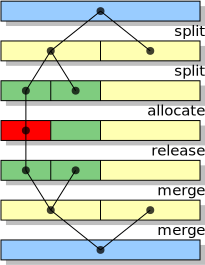
\includegraphics[width=0.30\textwidth]{build/alloc-free-cycle.eps}
\end{center}
\caption{Graficzna reprezentacja cyklu alokacji i~zwalniania buforów
  w~algorytmie bliźniaków.}
\end{wrapfigure}

Alokator stron implementuje algorytm bliźniaków (skąd też jego inna
angielska nazwa: {\it buddy system} lub {\it buddy allocator}), który
operuje na blakach o~rozmiarze $2^k$ jednostek.  W~przypadku Linuksa
jednostką jest pojedyncza strona fizyczna, a~na $k$~narzucone jest
ograniczenie $k < \mathrm{MAX\_ORDER}$.  \lstinline|MAX_ORDER| może
zależeć od architektury, na którą Linuks jest kompilowany, ale
zazwyczaj ma wartość $11$ (toteż na potrzeby tej pracy zakładam, iż $0
\le k \le 10$).

W~Linuksie, przez $k$ rozumie się rząd\TODO{może po prostu lepiej
  zostawić „order” i~nie tłumaczyć?} strony (\ang{page order}).
Strona rzędu 0 to pojedyncza strona fizyczna, strona rzędu 1
(\ang{1-order page}) to dwie strony fizyczne itd.\ aż do strony rzędu
10, czy też strony maksymalnego rzędu (\ang{max order page}), która
składa się z~1024 stron fizycznych.  Ogólnie, strona rzędu $n$ składa
się z~dwóch stron rzędu $n-1$.

Funkcja \lstinline|alloc_pages()|, która jest interfejsem dla
alokatora stron, przyjmuje jako argument właśnie rząd żądanej strony.

Z~powyższego opisu wynikają następujące właściwości alokatora stron.

\begin{itemize}
\item Nie można za jego pomocą zaalokować mniej niż jednej strony,
  tj.\ 4096 bajtów.
\item Interfejs zwyczajnie nie pozwala alokować obszarów, których
  rozmiar nie jest potęgą dwójki.
\item Gdyby jednak chcieć zaalokować taki obszar, wiązałoby się to
  z~potencjalnie dużą fragmentacją wewnętrzną.  Dla przykładu bufor
  dla kolorowej tekstury o~rozmiarze $512 \times 512$ pikseli
  wymagałby obszaru o~rozmiarze \unit[1]{MiB}, z~których
  \unit[256]{KiB}, a~więc \nicefrac{1}{4}, byłoby nieużywane.
\item Alokator stron nie jest w~stanie zaalokować obszaru większego
  niż \unit[4]{MiB}.  Z~tego powodu, nie nadaje się do alokowania
  ciągłego fizycznie buforu dla 5 megapikselowej kamery, czy nawet dla
  pojedynczej ramki {\it full HD}.
\end{itemize}

Jak zatem działa algorytm bliźniaków.  Alokator posiada listę wolnych
stron, których rząd jest pomiędzy $0$ a~$10$.  W~Linuksie zrealizowane
jest to poprzez 11 list dwukierunkowych, gdzie każda przeznaczona jest
dla stron o~konkretnym rzędzie.

Gdy sterownik chce zaalokować stronę rzędu $n$, alokator sprawdza
odpowiednią listę.  Jeżeli jest ona pusta, przechodzi do listy ze
stronami rzędu $n+1$, aż znajdzie wolną stronę (lub dojdzie do
maksymalnego rzędu, co sygnalizuje nieudaną alokacji.  Jeżeli uzyskana
w~ten sposób strona ma rząd większy niż żądany, jest ona dzielona na
pół, aż do osiągnięcia żądanego rozmiaru.  Strony, które powstały na
skutek podziału większej strony na pół, nazywamy stronami
bliźniaczymi.  Cały proces ilustruje algorytm \ref{alg:buddy-alloc}

\begin{algorithm}\label{alg:buddy-alloc}
\caption{Alokacja strony rzędu $k$ w~algorytmie bliźniaków}
\begin{algorithmic}[1]
\Require $0 \leq k < \mathrm{MAX\_ORDER}$
\Function{AllocatePage}{$k$}
    \State $i \gets k$
    \While {lista stron rzędu $i = \emptyset$}
        \State $i \gets i + 1$
        \If {$i = \mathrm{MAX\_ORDER}$}
            \State \Return $\emptyset$
        \EndIf
    \EndWhile

    \State $p \gets$ strona z listy stron rzędu $i$
    \While {$i \neq k$}
        \State $i \gets i - 1$
        \State podziel $p$ na pół na $p_1$ i $p_2$
        \Comment{Strony $p_1$ i $p_2$ nazywamy stronami bliźniaczymi}
        \State $p \gets p_1$
        \State dodaj $p_2$ do listy stron rzędu $i$
    \EndWhile
    \State \Return $p$
\EndFunction
\end{algorithmic}
\end{algorithm}

Przy zwalnianiu, dopóki to możliwe, strona jest łączona ze swoją
bliźniaczą stroną, dzięki czemu strony są dodawane do lista wolnych
stron o~dużym rzędzie.  Proces ten ilustruje algorytm
\ref{alg:buddy-free}

\begin{algorithm}\label{alg:buddy-free}
\caption{Zwalnianie strony $p$ rzędu $k$ w algorytmie bliźniaków}
\begin{algorithmic}[1]
\Procedure{FreePage}{$p$, $k$}
    \While {$k + 1 \neq \mathrm{MAX\_ORDER} \wedge p$ posiada wolną stronę bliźniaczą}
        \State $p' \gets$ strona bliźniacza $p$
        \State usuń $p'$ z~listy wolnych stron
        \State $k \gets k + 1$
        \State $p~\gets$ strona powstała w~wyniku połączenia $p$ i~$p'$
    \EndWhile
    \State dodaj $p$ do listy wolnych stron rzędu $k$\label{alg:buddy-free:add}
\EndProcedure
\end{algorithmic}
\end{algorithm}


\section{Typy migracji}\label{sec:migratetype}

Powyższy opis pomija niektóre szczegóły alokatora stron.  Po pierwsze,
nawet jeżeli w~danej chwili nie istnieje wolna strona o~żądanym
rzędzie, aktywowana jest tzw.\ wolna ścieżka (\ang{slow path}), która
wykorzystuje różne mechanizmy odzyskiwania pamięci (np.\ poprzez
zwalnianie buforów dyskowych, czy w~najgorszym przypadku zabiciu
jednego z~działających procesów).  Mechanizmy te nie są jednak istotne
dla tematyki niniejszej pracy i~dlatego zostały pominięte.

Ważnym czynnikiem są typy migracji (\ang{migratetype}), których jest
sześć: {\it unmovable}, {\it reclaimable}, {\it movable}, {\it cma},
{\it reserve} oraz {\it isolate}).

\begin{itemize}
\item Dla potrzeb tej pracy traktuję typy {\it unmovable}, {\it
  reclaimable} i~{\it reserve} jak jeden typ -- typ nieruchomy.  To
  uproszczenie wynika z~faktu, iż dla CMA-y istotne jest tylko
  rozróżnienie pomiędzy stroną ruchomą i~nieruchomą.
\item Strony które są typu ruchomego charakteryzują się tym, że ich
  adres fizyczny nie jest istotny, w~związku z~czym mogą być
  przeniesione w~inne miejsce pamięci RAM.
\item Typ cma jest nowym typem dodanym przez CMA i~jest opisany
  dokładniej w~podrozdziale \ref{sec:migrate-cma}
\item Typ {\it isolate} jest niejako pseudo-typem, gdyż jeżeli wolna
  strona ma taki typ, nie może ona zostać zaalokowana.  Więcej na
  temat sposobu w~jaki ten typ może być wykorzystywany opisuję
  w~podrozdziale \ref{sec:alloc-contig-range}
\end{itemize}

Jednym z~przykładów stron ruchomych są strony anonimowe działających
procesów.  Ponieważ program odwołują się do nich poprzez mapowania
wirtualne, o~ile tablice translacji zostaną uaktualnione, zawartość
strony może być przeniesiona w~dowolne miejsce.  Podobnie wygląda
sprawa z~buforami dyskowymi i~wieloma innymi strukturami, którymi
zarządza jądro.

Proces przenoszenia ruchomej strony z~jednego miejsca w~inne nazywa
się migracją i wykorzystywany jest między innymi przy obsłudze
hot-swapu pamięci, a~także w~trackie procesu zagęszczania (opisanego
w~\cite{bib:compaction}), którego celem jest zwiększenie liczby
dostępnych stron o~wysokich rzędach.

Wołając funkcję \lstinline|alloc_pages()|, typ migracji strony jest
przekazywany jako argument, co pozwala alokatorowi stron grupować
strony tego samego typu.  Jest to istotne, gdyż mechanizm zagęszczania
nie działa zbyt dobrze jeżeli strony ruchomy przelatywały się
z~pozostałymi stronami, które nie podlegają migracji.

\section{Grupy stron}

Grupowanie to realizowane jest poprzez podział pamięci na bloki
składające się z~\lstinline|pageblock_nr_pages| stron (czy też
równoważnie na bloki rzędu \lstinline|pageblock_order|).  Konkretne
wartości tych stałych zależą od architektury, no którą jądro zostało
skompilowane, jak i~opcji konfiguracyjnych wybranych w~trakcie
kompilacji.  Niemniej, przeważnie wartość tych stałych to odpowiednio
1024 (stron) i~(rząd) 10 i~właśnie takie są przyjęte w~tej pracy.

Każdy blok stron (\ang{pageblock}) ma przypisany typ migracji,
a~alokator stron posiada oddzielne listy wolnych stron dla każdego
typu migracji.  Zatem patrząc na algorytm \ref{alg:buddy-alloc} należy
zdawać sobie sprawę, iż rozpatruje on listy wolnych stron danego typu
migracji.

\section{Zmiana typu migracji}\label{sec:type-change}

Należy pamiętać, iż dla jądra zrealizowanie alokacji jest ważniejsze
od trzymania stron o~tym samym typie migracji razem.  Dlatego dla
każdego typu migracji istnieje list zapasowych (\ang{fallback}) typów
migracji.  Jeżeli alokacja dla żądanego typu migracji nie powiedzie
się, alokator stron będzie próbował z~kolejnymi typami z~list, tak jak
to pokazuje algorytm \ref{alg:buddy-fallback}

Co więcej, jeżęli rząd żądanej strony jest dostatecznie duży, typ
migracji wszystkich wolnych stron w~danym bloku stron zostaje
zmieniany na ten zgodny z~wywołąniem funkcji
\lstinline|alloc_pages()|.

\begin{algorithm}\label{alg:buddy-fallback}
\caption{Alokacja strony rzędu $k$ z~uwzględnieniem typu migracji $m$}
\begin{algorithmic}[1]
\Function{ChangeBlockMigrateType}{$b$, $m$}
\State zmień typ migracji $b$ na $m$
\ForAll {wolnych stron $p' \in b$}
    \State przenieś $p'$ na listę wolnych stron typu $m$
\EndFor
\EndFunction
\Statex
\Function{AllocPageMigrateType}{$k$, $m$}
    \State $f \gets$ lista zapasowych typów migracji dla typu $m$
    \State dodaj $m$ na początek $f$
    \ForAll{$m' \in f$}
        \State $p \gets$ \Call{AllocPage}{$k$} biorąc pod uwagę listy stron typu $m'$
        \If {$p \neq \emptyset$}
            \If {$m \neq m' \wedge k \geq \nicefrac{\mathrm{page\_order}}{2}$}
                \State $b \gets$ blok stron zawierający $p$
                \State \Call{ChangeBlockMigrateType}{$b$, $m$}
            \EndIf
            \State \Return $p$
        \EndIf
    \EndFor
    \State \Return $\emptyset$
\EndFunction
\end{algorithmic}
\end{algorithm}

Podczas zwalniania, gdy strona jest dodawana do listy wolnych stron
(wideczne w~linii \ref{alg:buddy-free:add} algorytmu
\ref{alg:buddy-free}) typ migracji listy, na którą strona trafia
determinowany jest poprzez typ migracji przypisany blokowi stron do
którego dana strona należy.

Istotne jest tutaj, aby zauważyć, iż bloki stron mogą zmieniać swój
typ migracji, a~także, że nawet jeżeli blok ma dany typ migracji,
strony o~innym typie migracji mogą być z~niego przydzielone.


\section{Listy PCP}

Ostatnim istotnym, z~punktu widzenia CMA, aspektem alokatora stron są
listy PCP.  Ponieważ listy wolnych stron są współdzielone w~obrębie
całego systemu dostęp do nich musi być synchronizowany pomiędzy
wszystkimi procesorami.  Aby uniknąć kosztów związanych
z~synchronizacją, każdy procesor posiada swoje prywatne PCP listy, na
których znajdują się wolne strony rzędu 0.  Biorąc również i~ten
aspekt pod uwagę, alokacja przyjmuje postać przedstawianą w~algorytmie
\ref{alg:buddy-pcp}

\begin{algorithm}\label{alg:buddy-pcp}
\caption{Alokacja strony rzędu $k$ z~typem migracji $m$
  z~uwzględnieniem list PCP}
\begin{algorithmic}[1]
\Function{AllocPageUsePCP}{$k$, $m$}
    \If {$k \neq 0$}
        \State $p \gets$ \Call{AllocPageMigrateType}{$k$, $m$}
    \Else
        \State $l \gets$ lista PCP dla typu migracji $m$
        \If {$l = \emptyset$}
            \State $i \gets 0$
            \Repeat
                \State $p \gets$ \Call{AllocPageMigrateType}{$0$, $m$}
                \If {$p \neq \emptyset$}
                    \State dodaj $p$ do $l$
                    \State $i \gets i + 1$
                \EndIf
            \Until {$i \geq n \vee p = \emptyset$} \Comment{Wartość
              $n$ jest zależna od różnych czynników}
        \EndIf
        \If {$l = \emptyset$}
            \State \Return $\emptyset$
        \Else
            \State $p \gets$ pierwsza strona z $l$
            \State usuń pierwszą stronę z $l$
            \State lista PCP dla typu migracji $m$ $\gets l$
        \EndIf
    \EndIf
    \State \Return $p$
\EndFunction
\end{algorithmic}
\end{algorithm}


\chapter{Contiguous Memory Allocator}\label{sec:cma}

Podstawowym założeniem CMA jest umożliwienie alokowania dużych
obszarów ciągłych fizycznie bez konieczneści rezerwacji na wyłączność
dużej ilości pamięci.  Aby to umożliwić, CMA korzysta z~mechanizmu
migracji stron opisanego w~podrozdziale \ref{sec:migratetype}.

\section{Typ migracji CMA}\label{sec:migrate-cma}

Migracja jest możliwa tylko dla stron ruchomych.  Niestety, przed
zaimplementowaniem CMA, w~Linuksie nie istniał mechanizm, który
pozwalałby zagwarantować, aby w~systemie istniał duży obszar, w~którym
strony są wolne albo ruchome.  Ponieważ (jak opisałem w~podrozdziale
\ref{sec:type-change}) jądro dopuszcza alokacje nieruchomych stron
z~bloków stron oznaczonych jako przechowujące strony ruchome, a~także
posiada mechanizm na skutek którego bloki stron zmieniają swój typ,
oznaczenie bloku stron jako ruchome nie gwarantuje, że tylko strony
ruchome będą alokowane z~tego bloku stron.

Z~tego powodu, aby CMA dobrze działała, pierwszym krokiem było
stworzenie nowego typu migracji, nazwanym po prostu typem migracji CMA
(\lstinline|MIGRATE_CMA|).  Typ ten posiada dwie bardzo istotne cechy:

\begin{itemize}
\item Z~bloków stron oznaczonych typem CMA mogą być alokowane tylko
  strony ruchome.  Innymi słowy, typ migracji CMA istnieje w~lista
  zaposowych typów migracji jedynie dla typu ruchomego.
\item Blok oznaczony typem CMA nie zmienia swojego typu (na skutek
  działania alokatora stron).
\end{itemize}

O~ile pierwsza właściwość jest stosunkowo prosta do osiągnięcia,
zagwarantowania niezmienności typu bloku stron wymagało
zidentyfikowaniem wszystkich sytuacji, w~których blok może zmienić
swój typ (a~także sytuacji, w~których strony mogą trafić na listy
wolnych stron dla typu niezgodnego z~typem bloku, do którego należą)
i~dodanie odpowiednich warunków zapewniających, że nieporządana zmiana
nie nastąpi.

\section{Alokowanie obszaru pamięci}\label{sec:alloc-contig-range}

W~sytuacji, gdy istnieje gwarancja, że dany zakres stron posiada
jedynie strony wolne i~ruchome, można przystąpić do jej alokacji.
Drugim krokiem implementowania CMA było zatem stworzenie funkcji,
które dostaje jako argument zakres stron, a~następnie migruje
wszystkie zajęte strony, a~wolne usuwa z~listy wolnych stron.

\begin{algorithm}\label{alg:alloc-contig-range}
\caption{Alokacja strony z~podanego zakresu}
\begin{algorithmic}[1]
\Function{AllocContigRange}{$s$, $e$}
    \State $s' \gets s$ wyrównane w~dół do płnej strony maksymalnego rzędu
    \State $e' \gets e$ wyrównane w~górę do płnej strony maksymalnego rzędu
    \State izoluj strony z~zakresu $\left< s', e' \right)$
    \State migruj zajęte strony z~zakresu $\left< s, e~\right)$
    \State wyczyść PCP listy
    \ForAll{$p \in $\left< s', e' \right)$}
        \State usuń $p$ z listy wolnych stron
    \EndFor
\EndFunction
\end{algorithmic}
\end{algorithm}



\appendix

\nocite{*}
\bibliographystyle{plplain}
\begin{thebibliography}{9}

%% \bibitem{bib:ldd3}
%%   J. Corbet, A. Rubini i G. Kroah-Hartman,
%%   \emph{Linux Device Drivers, Third Edition}.
%%   2005.
%%   \url{http://lwn.net/Kernel/LDD3/}

\bibitem{patch:cma-24}
  M.Nazarewicz i~M. Szyprowski,
  \emph{Contiguous Memory Allocator, v.\ 24},
  3 kwietnia 2012.
  \url{http://thread.gmane.org/gmane.linux.kernel.mm/76241}

\bibitem{patch:pmm}
  M. Nazarwicz,
  \emph{Physical Memory Management}.
  13 maja 2009.
  \url{http://lkml.org/lkml/2009/5/13/100}

\bibitem{patch:cma-4}
  M. Nazarewicz,
  \emph{The Contiguous Memory Allocator framework, v.\ 4},
  20 sierpnia 2010.
  \url{http://thread.gmane.org/gmane.linux.kernel.mm/52010}

\bibitem{patch:bigphys}
  D. Tochansky,
  \emph{bigphysarea patch for 3.2.x},
  27 marca 2012.
  \url{http://article.gmane.org/gmane.linux.kernel/1273100}

%% \bibitem{bib:state-of-allocators}
%%   D. Rientjes,
%%   \emph{Status of the Linux Slab Allocators}.
%%   Southern California Linux Expo, February 26, 2011
%%   \url{http://www.socallinuxexpo.org/scale9x/presentations/status-linux-slab-allocators.html}

\end{thebibliography}


\end{document}
